\section{Previous Research}
\label{Previous_Research}
This section summarizes four important papers, which all have made a big impact in the area of deep reinforcement learning. Each paper is described with the important concepts in the represented paper. It will give a overview of state of the art in the area of deep reinforcement learning.   

\subsection{Playing Atari with Deep Reinforcement Learning }\cite{DBLP:journals/corr/MnihKSGAWR13}
This paper was published in 2013 by DeepMind Technologies. It is the first paper to make a deep learning model to successfully learn control policies directly from sensory input using reinforcement learning. 

The paper present some of the challenges by using deep learning to do reinforcement learning. One of the challenges is deep learning algorithm requires large amount of handlabelled training data. Another challenge is the delay between action and resulting reward, which can be thousands timesteps long.The paper demonstrates that a convolutional neural network can overcome these challenges. 

The goal is to connect a reinforcement learning algorithm to a deep neural network which uses RGB images and process training data by using stochastic gradient update. The starting point for this approach is to use Tesauro's TD-Gammon \cite{Tesauro:1995:TDL:203330.203343} architecture. The network is different from TD-Gammon and other online approaches, because it uses a technique known as experience replay, where the agent store the agents experiences at each time-step.

The input to the neural network is an $84 x 84 x 4$ image. The output from the neural network is a single output for each valid actions. The architecture of the network can be seen on \Cref{fig:playing_atari}   
\begin{figure}[H]
	\centering
	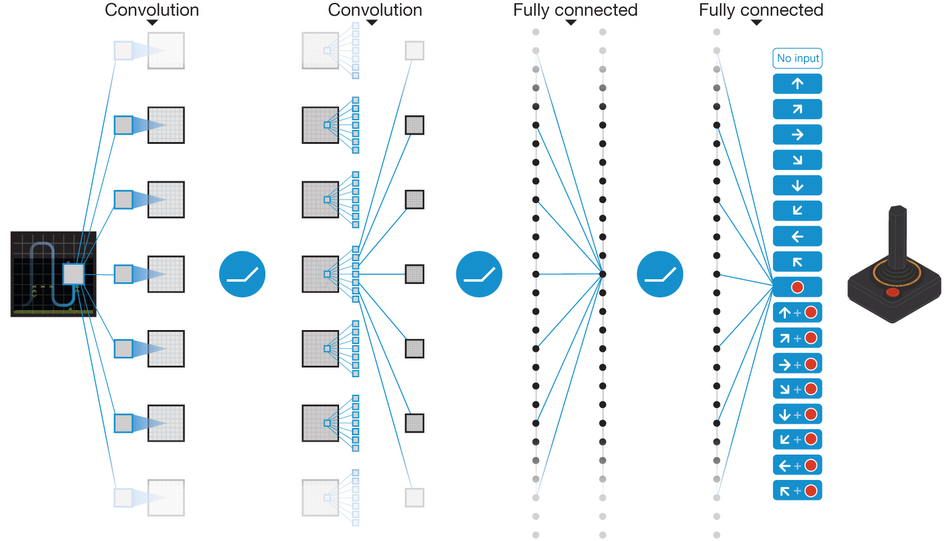
\includegraphics[width=0.7\textwidth]{Figures/TheoreticalBackground/playing_atari.jpg}
	\caption{The arhitecture of the network used in the article "Playing Atari with Deep Reinforcement Learning"}
	\label{fig:playing_atari}
\end{figure} 

This network is tested on seven Atari games, and the approach in this paper gave state-of-the-art result in six of the seven games. Finally it showed better performance than a expert human player in three out of the seven games.  

\subsection{Mastering the Game of Go with Deep Neural Networks and Tree Search}\cite{Silver_2016}
This paper introduce a new approach to compete in the classic game Go, the paper was published in 2016. The game of Go is the most challenging classic game for artificial intelligence, due to the enormous search space and the difficulty of evaluating board positions and moves. 

They employ a similar architecture as in \cite{DBLP:journals/corr/MnihKSGAWR13}. Here they pass in the board position as a $19 x 19$ image and use convolutional layers to construct a representation of the position. It uses neural networks to reduce the search space, this is done by use of value networks to evaluate board position and policy networks to select moves.

The way they trained the Neural Network started with training a supervised learning policy network, directly from expert human moves. Next training the reinforcement learning policy network is done by improving the supervised learning network by optimizing the final outcome of games og self-play. The final atep of training, is to train the value network, that predict the winner of the games played by the reinforcement learning policy network against it self.   

By combining tree search with policy and value networks, \textit{AlphaGo} has reached a professional level in Go. In March 2016 \textit{AlphaGo} won 4-1 against the legendary Lee Sedol , the top Go player in the world over the past decade.  

\subsection{Asynchronous Methods for Deep Reinforcement Learning}\cite{DBLP:journals/corr/MnihBMGLHSK16}
This is another paper from the team behind \cite{DBLP:journals/corr/MnihKSGAWR13}, and was published in 2016. This paper provide a very different paradigm for deep reinforcement learning. Instead of experience replay, it asynchronously execute multiple agents in parallel, on multiple instances of the environment. 

This simple idea enables much larger spectrum of on-policy reinforcement learning algorithm as well as off-policy reinforcement learning algorithm, to be applied robustly and effectively using deep neural networks.  It also offers practical benefits, this experiment is able to run on a single machine with a standard multi-core CPU, instead of specialized such as GPUs.

The paper presents asynchronous versions of four standard reinforcement algorithms used on different platforms. The platform used is a simulator for Atari 2600, Torcs 3D car racing simulator, Mujoco and Labyrinth. The asynchronous advantage actor-critic (A3C) algorithm was the best performing agent on all the platforms.

The asynchronous advantage actor-critic (A3C) beats state of the art result in 26 of 57 Atari games. This is a big improvement from previously reinforcement networks. When trained on the Atari domain using 16 CPU cores, the proposed asynchronous algorithm train faster than Deep Q-Network trained on an Nvidia K40 GPU, with A3C surpassing the state of the art in half the training time.   

\subsection{Deep Reinforcement Learning framework for Autonomous Driving} \cite{Sallab:2017:2470-1173:70}
This paper is motivated by the papers \cite{DBLP:journals/corr/MnihKSGAWR13} and \cite{Silver_2016}. It propose a framework for autonomous driving using deep reinforcement learning, the paper was published in 2017. It is relevant because it is difficult to handle autonomous driving as a supervised learning problem due to interactions with the environment. It also integrates recent work on attention models, to focus on relevant information, thereby reducing the computational complexity.

They propose a framework for an end-end autonomous driving model that takes in raw sensor input and output the driving actions. The model is able to handle partially observable scenarios. 

The framework can be seen on \Cref{fig:Framework_article}. In the model the spatial features are extracted via a CNN, which learns the features from data. To Decode the true environment state a LSTM network is used, which are able to control which information to keep from previous state. The final part of the framework is the reinforcement planing part. The inputs are the states of the environment and their aggregations over time. The output of the framework is the driving actions. 

The paper used The Open-source Racing Car Simulator (Torcs) with a lane keeping assist algorithm to test the framework. The result is a successful lane keeping behavior with speed limit.    

\begin{figure}[H]
	\centering
	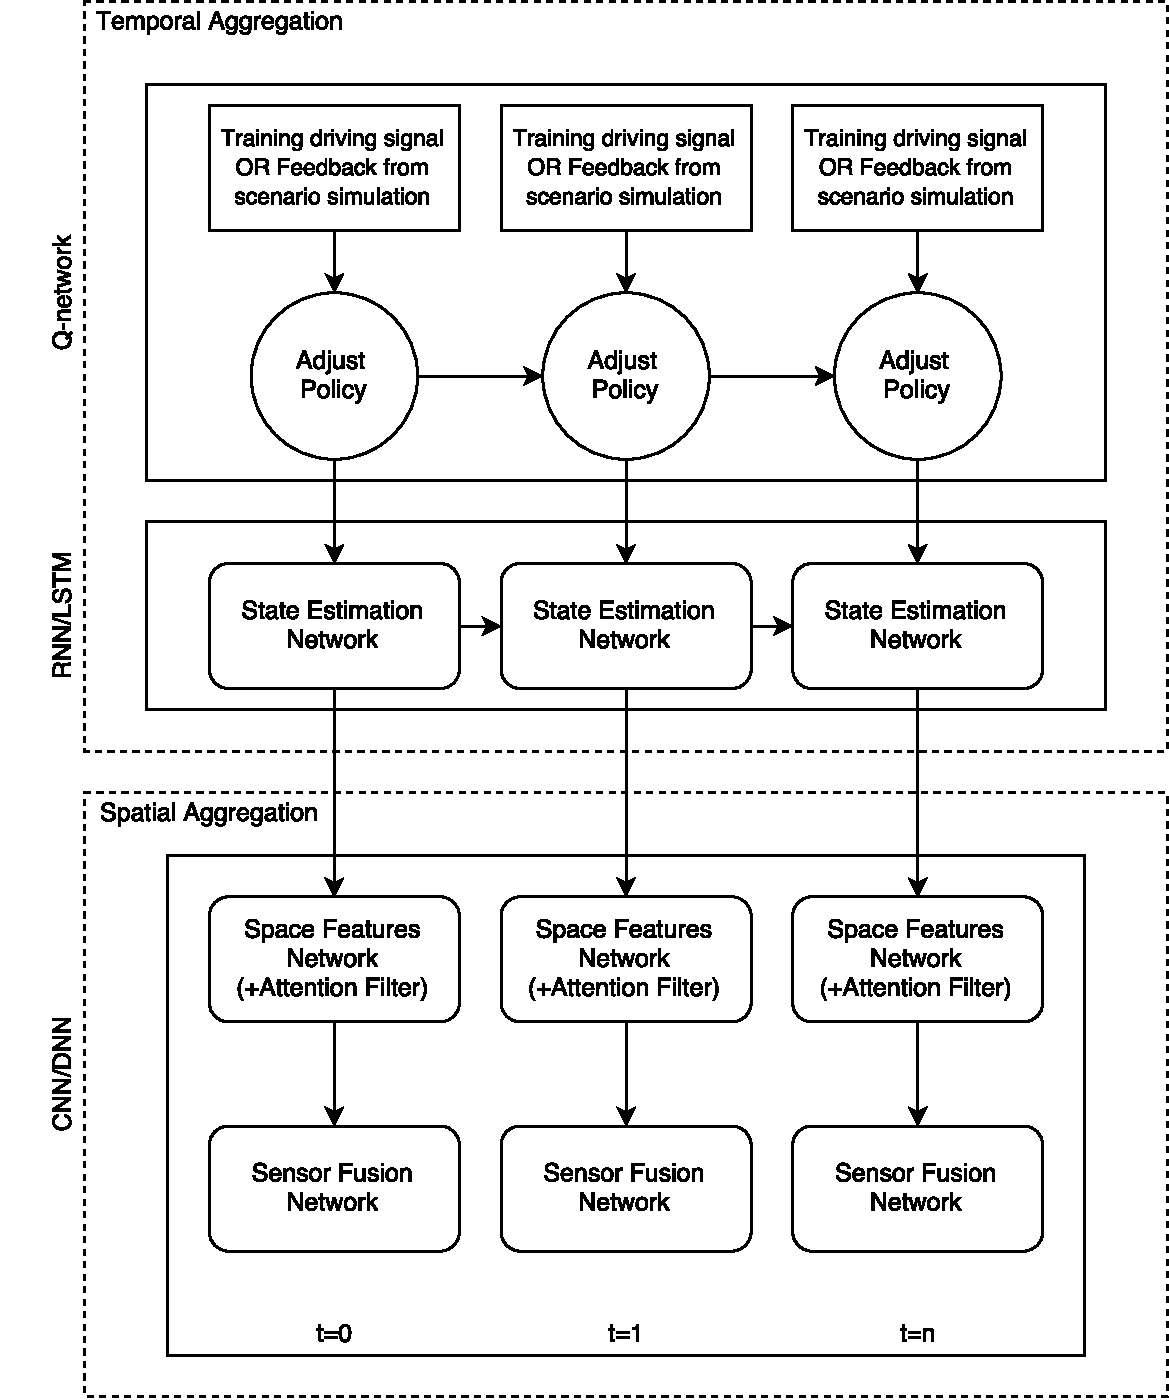
\includegraphics[width=0.8\textwidth]{Figures/TheoreticalBackground/Framework_article}
	\caption{Framework from the article "Deep Reinforcement Learning framework for Autonomous Driving}
	\label{fig:Framework_article}
\end{figure}
 